 In figure\ \ref{fig:ExpModelBlocks}, the main steps of this work 
 are portrayed.


 \begin{figure}[H]
    \centering
    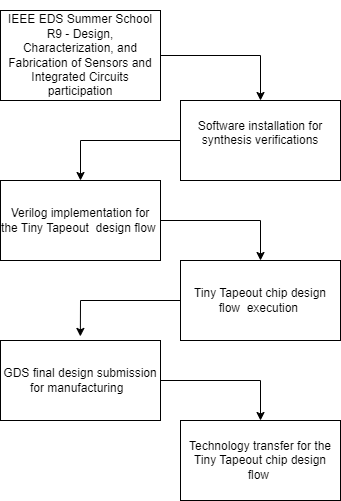
\includegraphics[width=\linewidth]{Pictures/ExperimentalModel.png}
    \caption{Experimental Model Blocks}
    \label{fig:ExpModelBlocks}
\end{figure}

\subsection{IEEE EDS Summer School R9 \- Design, Characterization, and Fabrication of Sensors and Integrated Circuits participation}
In June 2023 two senior students from the Electronics Engineering department at Universidad del Valle de Guatemala were granted scholarships 
to attend the ``2023 IEEE EDS Summer School R9" in Puebla, Mexico Throughout this enlightening summer program, a wide array of topics were 
addressed, ranging from insights of former students who work in the field, to several educational tools provided by one of the industry leaders; 
Synopsys. A significant message stood out: Nanochip design and fabrication industry is so complex, so dynamic, and so expensive due to infrastructure, 
human resources, etc. so that it becomes extremely challenging to almost impossible for academia to keep up with it.
During the program, the gap between industry capability and academic resources became evident as the alumni shared their experiences. 
Some of the former students highlighted that they had encountered setbacks in their projects due to challenges in installation or upkeep of some 
tools within the expansive realm of semiconductor technology. Notably, a few even mentioned that a lack of infrastructure and limited time had led to the 
unfortunate loss of grants they had secured for their projects.In the program, there were also discussions about new open-source tools such as Wokwi, 
designed to facilitate learning about logical circuitry. The Efabless initiative was another topic, that was introduce as a private semiconductor fabrication 
company, but the one that left the most significant impact was Tiny Tapeout because it closes de gap between the complexity behind the chip design and manufacturing 
in industry and the resources, time, and knowledge typically available in academia. This tool stood out for its adoption is further supported by a multi-purpose wafer 
and the cost-effectiveness of chip production. Typically, one of the challenges in academia involves acquiring the necessary computing power to run complex design tools. 
However, Tiny Tapeout has tackled this issue by providing its own cloud computing infrastructure, effectively reducing the demand for high computational resources. On 
the other hand, the installation of some of the highly advanced programs use in the industry are very complex using authentication servers to secure their tools, 
however Tiny Tapeout has manage to set their installation tool process very straightforward using only three steps. It’s worth mentioning that Tiny Tapeout has its 
own website where you can consult any doubt its installer might have, and it has several channels of communication. The aim of the Tiny Tapeout initiative is not 
to take over the semiconductor industry but to give students the knowledge and experience of working in this ample field, moreover, offer students the experience of taking a digital design all the way to semiconductor fabrication.


\subsection{Software installation for synthesis verifications}

To verify that both logical and physical synthesis align with the Verilog files, the installation of an  open-source integrated circuit design flow called OpenLane was performed. To use it, a virtual machine with Ubuntu 22 was set up, and the necessary prerequisites, including Python 3, git, make, and Docker, were installed. The GitHub repository containing OpenLane was cloned and compiled. It was confirmed that OpenLane operated correctly by synthesizing a 4-bit adder.
 

\subsection{Verilog implementation for the Tiny Tapeout design flow}
% Daniel 
This section introduces the Verilog implementation within the framework of Tiny Tapeout, a project dedicated to generating chip layouts from Verilog files. In this context, we will delineate the four distinct designs produced, providing comprehensive descriptions of the modules and their respective behaviors.

\subsubsection{Multi stage path for delay measurements}
The core of the module featured an approach to creating a ring oscillator. Although it was initially intended to utilize cascaded NOT gates, it was observed that the synthesizer, under the constraints of the Tiny Tapeout design flow, may replace these gates with buffers. As a result, the oscillatory behavior was expectedly altered. Nevertheless, the module's ring oscillator function was realized through a sequence of logical operations involving AND gates and inverters, forming a feedback loop. The logical signals EN and EN\_2 served as inputs to an AND\_2 module, generating a waveform represented by W\_1. Subsequently, this waveform traversed a series of inverters (tt\_prim\_inv modules), resulting in the generation of W\_2, W\_3, and cyclically returning to W\_1. While this configuration may not conform precisely to the original design intent, it offers a valuable educational opportunity to explore gate delays and their implications in digital circuitry when compared to theoretical calculations.\\

\subsubsection{ASCII Text Printer Circuit}
A Verilog module was designed to function as a text printing system capable of displaying two distinct texts, which are selected through an external signal. The module employs an internal counter synchronized with the clock to determine the specific ASCII character displayed based on the selection signal and the counter value. The output is provided through the output pins in ASCII format.\\

\subsubsection{Implementation of the Pong game}
The Verilog code, pong\_neopixel.v, with the main module "tt\_um\_pong\_neopixel", has been 
developed with the purpose of implementing a version of the Pong game on a Neopixel pixel 
matrix. This design has been conceived as an example of an interactive and playful application 
of programmable digital hardware. The "tt\_um\_pong\_neopixel" module consists of several 
inputs and outputs intended to control the game, including player input signals, start 
signals, and outputs to manage the Neopixel matrix, along with clock and reset signals. To 
ensure the stability of the input signals, "debounce" modules have been implemented. The game 
logic includes the management of the movement of the players' paddles and the ball, as well as 
collision detection and game reset when appropriate. In addition, logic has been developed to 
generate Neopixel signals that control the display on the matrix, allowing player interaction. 
This design also incorporates counters to track the sending of data to the matrix and 
appropriately selects whether LEDs should be turned on or off based on the position of the 
ball and paddles.\\

\subsubsection{Pulse Width Modulation Generator}
The Verilog code, pwm\_generator.v, with the main module "tt\_um\_pwm", is designed to 
generate a pulse width modulation (PWM) signal controlled by buttons. The module allows the duty cycle of the PWM signal to be increased or 
decreased via buttons. To ensure a reliable reading of the buttons, debounce logic is implemented that 
generates a slow clock signal (slow\_clk\_enable).\\
\subsection{Tiny Tapeout chip design flow execution}
% Daniel 
The execution of the Tiny Tapeout chip design flow begins with a series of essential steps. First it is necessary to fork the example repository provided by the Tiny Tapeout project. Once this step is completed, enabling the repository's capability to perform actions is crucial, as it allows for the automation of subsequent processes. To ensure the project's proper execution, several key tasks must be carried out. First all Verilog files must be located in the "src" folder. Additionally, the "info.yaml" file must be filled out with relevant information, including the Verilog files that constitute the design, the main design module, the authors, a project description, and, if applicable, the clock frequency. These steps are fundamental to ensuring an effective design flow and the correct implementation of chips in Tiny Tapeout.
\subsection{GDS final design submission for manufacturing}

In the final submission phase of the GDS design for 
manufacturing, a series of crucial steps were undertaken to ensure the
integrity and accuracy of the delivered information. First a comprehensive 
review of all relevant repositories was conducted with the aim of identifying
and rectifying any errors that may have existed in their execution. Subsequently
the provided form by Latin Practice was completed, requiring essential 
details about the repositories, including author names and direct links 
to the referred repositories. It is noteworthy that this form-filling 
process was rigorously carried out before the stipulated deadline, which 
was September 5th. These steps were taken to ensure the consistency and 
precision of the information provided in this critical stage of the GDS 
design project. In figures\ \ref*{fig:pwm_verified},\ \ref*{fig:pong_verified},
\ \ref*{fig:ascii_verified}, and\ \ref*{fig:delay_verified} the verification 
process of the four design sent to manufacture is shown to be successful.

\begin{figure}[tbh]
    \centering
    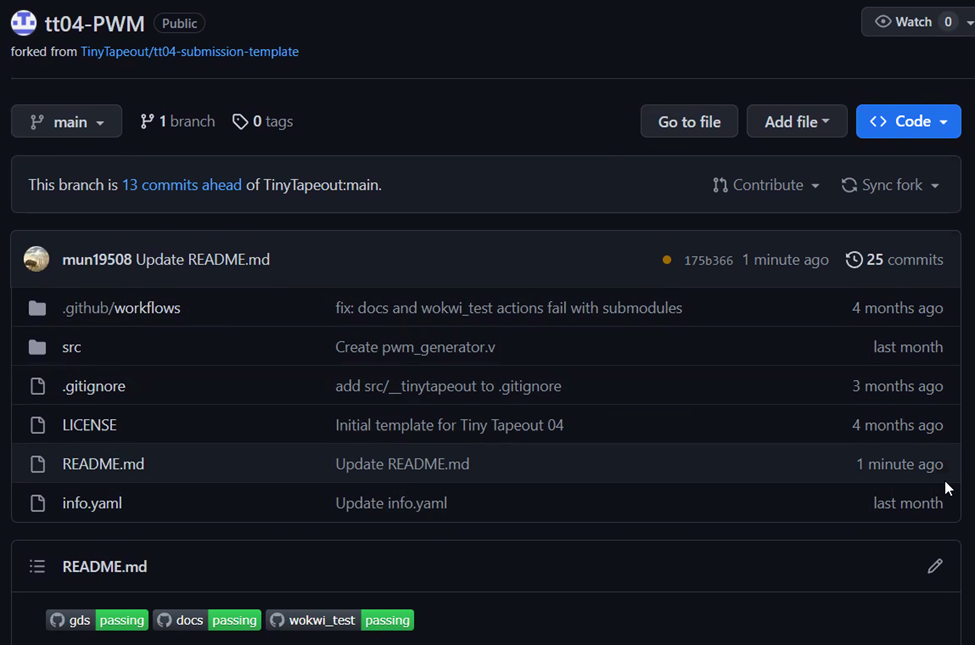
\includegraphics[width=\linewidth]{Pictures/pwm_verified.png}
    \caption{Verified Pulse Width Modulation Generator Verilog }\label{fig:pwm_verified}
\end{figure}

\begin{figure}[tbh]
    \centering
    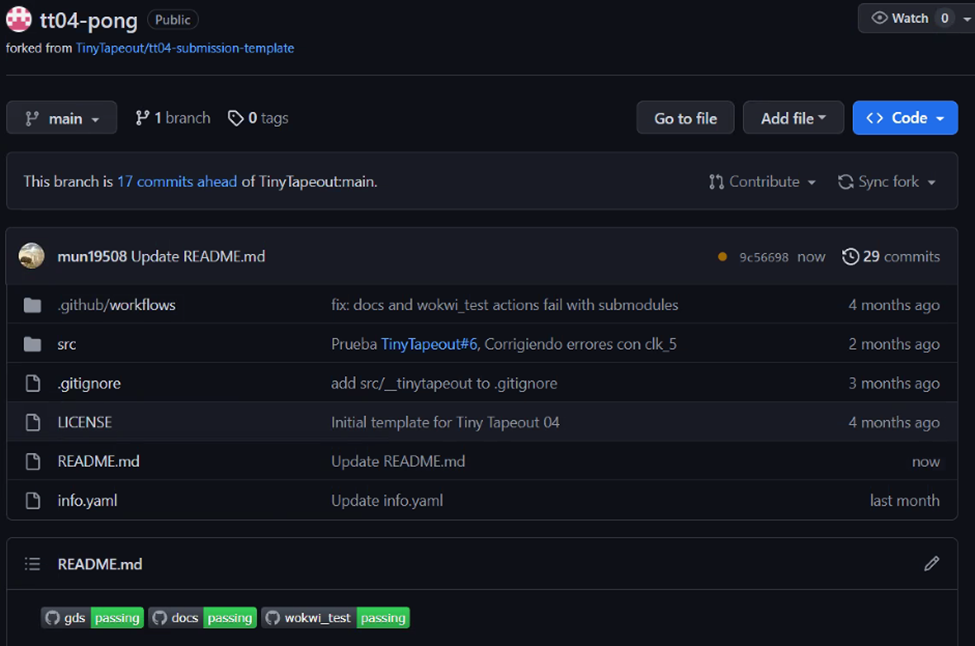
\includegraphics[width=\linewidth]{Pictures/pong.png}
    \caption{Verified Pong game Verilog}\label{fig:pong_verified}
\end{figure}

\begin{figure}[tbh]
    \centering
    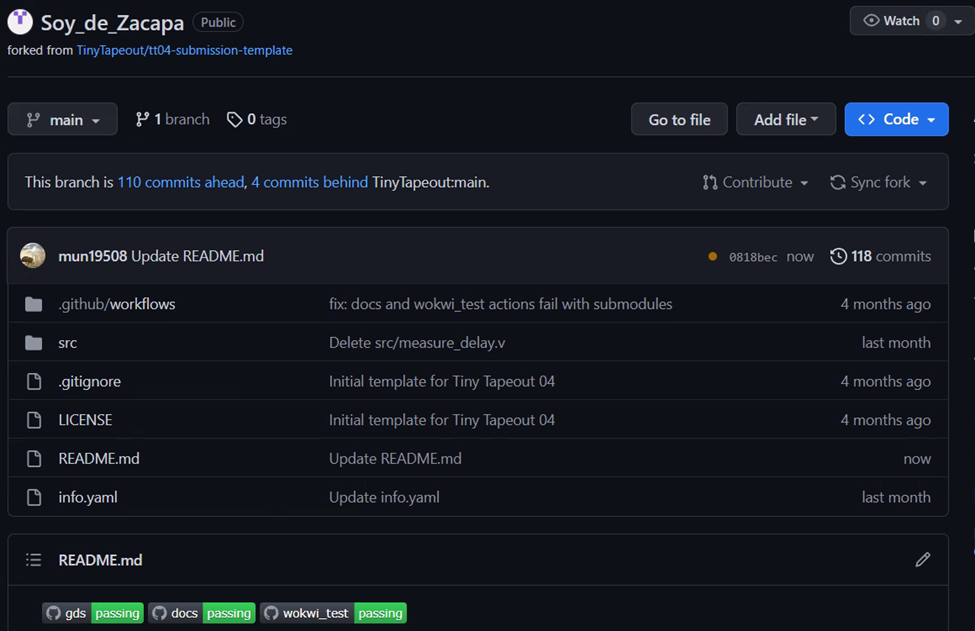
\includegraphics[width=\linewidth]{Pictures/verifide_zacapa.png}
    \caption{Verified ASCII Text Printer Circuit Verilog}\label{fig:ascii_verified}
\end{figure}

\begin{figure}[H] 
    \centering
    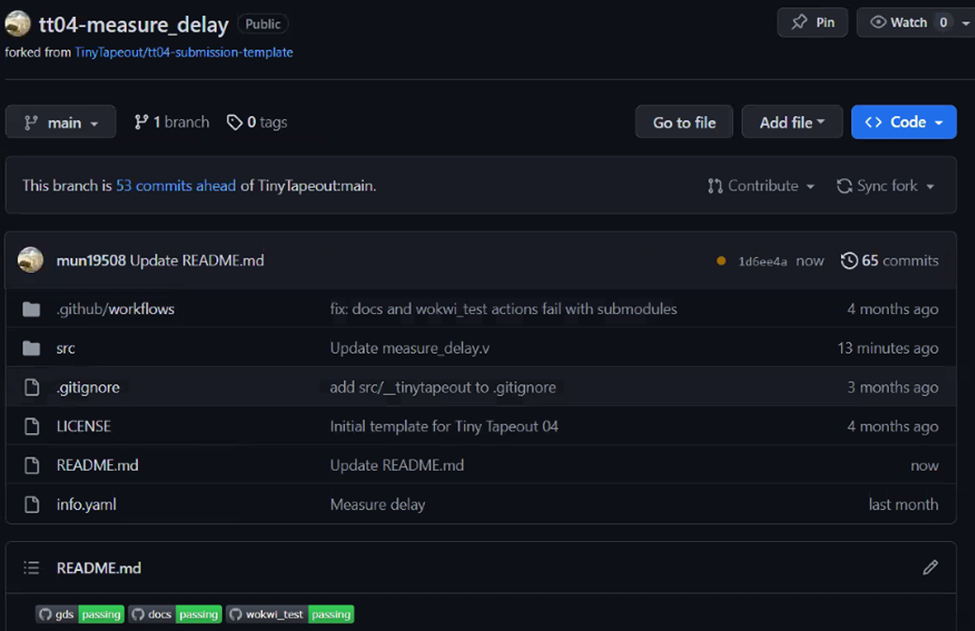
\includegraphics[width=\linewidth]{Pictures/delay_ver.png}
    \caption{Verified Multi stage path for delay measurements Verilog}\label{fig:delay_verified}
\end{figure}

\subsection{Technology transfer for the Tiny Tapeout chip design flow}

The true purpose behind this paper is to push the boundaries of understanding the semiconductor fabrication field at Universidad del Valle de Guatemala. The proper documentation of the knowledge acquired by all the members that were involved on this work is essential for future students. Therefore, Video tutorials and documents were made for students to replicate the Tiny tapeout program to take any design from a fully digital verilog implemented circuit all the way to a physical integrated circuit. 

% needed in second column of first page if using \IEEEpubid
%\IEEEpubidadjcol